\newpage 
\section{Auswertung}

\noindent
Im Folgenden werden die Kenngrößen verschiedener Operationsverstärkeraufbauten untersucht.
Außerdem werden auch Eigenschaften wie das Integrieren einer Eingangsspannung oder das generieren eines Signals betrachtet.


\subsection{Invertierter Linearverstärker}

\noindent
Für den invertierten Linearverstärker wurden die Amplituden des Eingangssignals $U_\t{E}$ und des Ausgangssignals $U_\t{A}$ für drei verschiedene Verstärkungsfaktoren $V$ aufgenommen.
Dies ergibt die theoretischen Leerlaufverstärkungen
\begin{align*}
  V_\t{1,theo}&= \frac{R_2}{R_1} &=\;\; \frac{\SI{10e3}{\ohm}}{\SI{1e3}{\ohm}} &= \num{10}\\
  V_\t{2,theo}&                  &= \frac{\SI{100e3}{\ohm}}{\SI{1e3}{\ohm}} &= \num{100}\\
  V_\t{3,theo}&                  &=\;\; \frac{\SI{68e3}{\ohm}}{\SI{1e3}{\ohm}} &= \num{68} \; . 
\end{align*}
Die mit den Messreihen korrespondierenden Messwerte sind in den Tabellen \ref{tab:lin1}, \ref{tab:lin2} und \ref{tab:lin3} dargestellt. 
Grafisch sind die mit $V_1$ korrespondierenden Messwerte in Abbildung \ref{fig:lin1} doppelt-logarithmisch aufgetragen.
Dabei sind die Werte, für die der Verstärkungsfaktor ungefähr konstant ist, eingezeichnet.
Über das Mitteln dieser Werte berechnet sich die Leerlaufverstärkung zu
\begin{equation*}
  V_1 = \SI{ 10.27(13)}{}
\end{equation*}
berechnen. Die Abweichung ergibt sich dabei über die Standardabweichung
\begin{equation*}
  \Delta x =  \sqrt{\frac{1}{n} \sum_{i \, = \, 1}^{n} \, \left(\bar{x}- x_i\right)^2}\; .
\end{equation*}
Auf der Flanke eingezeichneten Messwerte wird ein linearer Fit der Form 
\begin{equation*}
  V(f) = m \cdot f + n
\end{equation*}
berechnet. Da die Linearität allerdings bei doppelt-logarithmischen Daten auftritt, ergibt sich für die Fit-Funktion
\begin{equation}
  \ln(V) = m \cdot \ln\left(\frac{f}{\si{\hertz}}\right) + n \; .
  \label{eqn:lin} 
\end{equation}
Die Fitparameter errechnen sich damit zu 
\begin{align*}
  m &= \SI{-0.59 (5)}{}\\
  n &= \SI{ 8.04(59)}{} \; .
\end{align*}
Über diese lässt sich die Grenzfrequenz $f_\t{Grenz}$ bestimmen, bei der der Verstärkungsfaktor den Wert $\frac{V_\t{i}}{\sqrt{2}}$ annimmt.
Für $f_\t{Grenz}$ gilt damit
\begin{align*}
  \ln{\left(\frac{V_\t{i}}{\sqrt{2}}\right)} &= m \cdot \ln{\left(f_\t{Grenz,i}\right)} + n \\
  \iff f_\t{Grenz,i} &= \exp{\left( \ln\left( \frac{\frac{V_\t{i}}{\sqrt{2}} - n}{m}  \right)   \right)}\\
  f_\t{Grenz,i} &= \SI{27.05(3570)}{\kilo\hertz} \; .% in wirklichkeit \SI{27.05(3570)}{\kilo\hertz}
\end{align*}
Des Weiteren wird noch das Bandbreitenprodukt, zu
\begin{equation*}
  V_1 \cdot f_\t{Grenz,1} = \SI{277.84(36665)}{\kilo\hertz} % \SI{277.84(36665)}{\kilo\hertz}
\end{equation*} 
bestimmt. 
Die große Abweichung bei der Grenzfrequenz lässt sich vermutlich auf den großen Einfluss der Fehlerfortpflanzung 
über das Exponentieren, Logarithmieren und Dividieren in der Berechnung zurückführen.

\begin{figure}[H]
    \centering
    \includegraphics[width=0.6\textwidth]{build/plots/lin1.pdf}
    \caption{Die Messwerte des Verstärkungsfaktors des invertierenden Linearverstärkers für 
    $V_\t{1,theo}$ doppelt-logarithmisch aufgetragen.}
  \label{fig:lin1}
\end{figure}

\noindent
Das Vorgehen wird analog für den Verstärkungsfaktor $V_2$ durchgeführt. 
Die Messdaten und die für die einzelnen Auswertungen genutzten Datenbereiche sind in Abbildung \ref{fig:lin2} grafisch dargestellt.
Für die gemittelte Leerlaufverstärkung ergibt sich 
\begin{equation*}
  V_2 = \SI{96.00(115)}  \; .
\end{equation*}
Die Fitparameter des Flanken-Fits errechnen sich zu 
\begin{align*}
  m &= \SI{-1.01 (5)}{}\\
  n &= \SI{ 13.03(55)}{} \; .
\end{align*}
Daraus folgt für die Grenzfrequenz und das Bandbreitenprodukt
\begin{align*}
  f_\t{Grenz,2} &= \SI{63.34 (4404)}{\kilo\hertz}\\ % \SI{6334 (4404)}{\kilo\hertz}
  V_2 \cdot f_\t{Grenz,2} &= \SI{608.15(42278)}{\kilo\hertz} \; .%\SI{608.15(42278)}{\kilo\hertz} \; .
\end{align*}

\begin{figure}[H]
  \centering
  \includegraphics[width=0.6\textwidth]{build/plots/lin2.pdf}
  \caption{Die Messwerte des Verstärkungsfaktors des invertierenden Linearverstärkers für 
  $V_\t{2,theo}$ doppelt-logarithmisch aufgetragen.}
\label{fig:lin2}
\end{figure}

\noindent
Für den Verstärkungsfaktor $V_3$ werden wieder dieselben Faktoren bestimmt. 
Dabei ist die grafische Darstellung in Abbildung \ref{fig:lin2}.
Für die gemittelte Leerlaufverstärkung ergibt sich 
\begin{equation*}
  V_3 = \SI{67.45(140)} \; .
\end{equation*}
Die Fitparameter des Flanken-Fits errechnen sich zu 
\begin{align*}
  m &= \SI{-1.01 (4)}{}\\
  n &= \SI{ 13.14(48)}{} \; .
\end{align*}
Damit ergibt sich für die Grenzfrequenz und das Bandbreitenprodukt
\begin{align*}
  f_\t{Grenz,3} &= \SI{ 94.92(5861)}{\kilo\hertz}\\ % \SI{94.92(5861)}{\kilo\hertz}
  V_3 \cdot f_\t{Grenz,3} &= \SI{640.26(39513)}{\kilo\hertz} \; .%\SI{640.26(39513)}{\kilo\hertz}} \; .
\end{align*}


\begin{figure}[H]
  \centering
  \includegraphics[width=0.6\textwidth]{build/plots/lin3.pdf}
  \caption{Die Messwerte des Verstärkungsfaktors des invertierenden Linearverstärkers für 
  $V_\t{3,theo}$ doppellogarithmisch aufgetragen.}
\label{fig:lin1}
\end{figure}

\noindent
Zuletzt wird in Abbildung \ref{fig:phase} die Phasendifferenz zwischen Eingangs- und Ausgangsspannung für die verschiedenen Leerlaufverstärkungen dargestellt.
Die Phasenverschiebung folgen dabei der Form einer Sigmoid- oder $\t{arccot}$-Funktion.

\begin{figure}[H]
  \centering
  \includegraphics[width=0.6\textwidth]{build/plots/lin_phase.pdf}
  \caption{Die Messwerte der Phasenverschiebung für die Verstärkungsfaktoren $V_1 = 10 $, $V_2 = 100$ und $V_3 = 67$ 
  des invertierenden Linearverstärkers gegen die Frequenz aufgetragen.}
\label{fig:phase}
\end{figure}

\subsection{Umkehrintegrator}

\noindent
Für den Umkehrintegrator wurde ein Widerstand $R_1 = \SI{10}{\kilo\ohm}$ und ein Kondensator mit der Kapazität $C = \SI{100}{\nano\farad}$ verwendet.
Die aufgenommenen Messwerte der Eingangs- und Ausgangsspannung, die damit korrespondierenden Frequenzen und Phasen sind in Tabelle \ref{tab:int} zu finden.
Für die Auswertung wurden aus den Spannungen die Verstärkungsfaktoren berechnet und diese über die Frequenz $f$ gegen die Kreisfrequenz $\omega = 2\pi f $ doppelt-logarithmisch aufgetragen.
Dies ist in Abbildung \ref{fig:int1} dargestellt. 
Auf die dargestellten Messdaten wird nach Gleichung \ref{eqn:lin} eine Ausgleichsrechnung durchgeführt. 
Dabei soll die Proportionalität zum Inversen von $\omega$ für den Integrator und zu $\omega$ für den Differenzierer gezeigt werden. 
Außerdem soll der Faktor $RC$ identifiziert werden. 
Für den Koeffizienten-Vergleich muss die Fit-Funktion umgestellt werden.
\begin{align*}
  \ln(V) &= m \cdot \ln\left(\frac{\omega}{\si{\hertz}}\right) + n \\
  \implies V & = \exp\left(m\cdot \ln(\omega)\right)\cdot \exp\left(n\right)\\
  V &= \omega^m \cdot \exp\left(n\right)
\end{align*}
Im Vergleich mit den Gleichungen \ref{eqn:int} und \ref{eqn:dif} zeigt sich, dass für den Integrator 
\begin{align}
  m \approx -1 && \text{und} && \exp(n)= \frac{1}{RC}\label{eqn:int_RC}\\
  \intertext{gelten muss. Für den Differenzierer gilt}
  m \approx 1 && \text{und} && \exp(n)= RC\; . \label{eqn:dif_RC}
\end{align}
Für den in Abbildung \ref{fig:int1} dargestellten Fit wurden die Parameter
\begin{align*}
  m&=\SI{-0.81(2)}{}\\
  n&= \SI{5.83(11)}{}\\
  RC_\t{Int} &= \SI{2.9(3)}{\milli\second}\; .
\end{align*}
errechnet. Der theoretische Wert 
\begin{equation*}
  RC_\t{Theo,Int} = \SI{1}{\milli\second} 
\end{equation*}
ist dabei über die Proportionalität auch abgebildet.
\begin{figure}[H]
  \centering
  \includegraphics[width=0.6\textwidth]{build/plots/integrator.pdf}
  \caption{Die Messwerte des Verstärkungsfaktors des Umkehrintegrators gegen die Kreisfrequenz aufgetragen.
  Des Weiteren ist noch eine Theoriekurve und der Fit eingezeichnet.}
\label{fig:int1}
\end{figure}


\noindent
In den Abbildungen \ref{fig:int_sin}, \ref{fig:int_dre} und \ref{fig:int_recht} sind die Ausgabe des Oszilloskop 
für eine Sinus-, Dreieck- und Rechteck-Eingangsspannung dargestellt.
Dabei ist zu erkennen, dass wie erwartet die Sinusspannung zu einer Kosinusspannung integriert wurde, 
die Dreiecksspannung zu einer Sinusspannung und die Rechteckspannung zu einer Dreiecksspannung.

\begin{figure}[H]
  \centering
  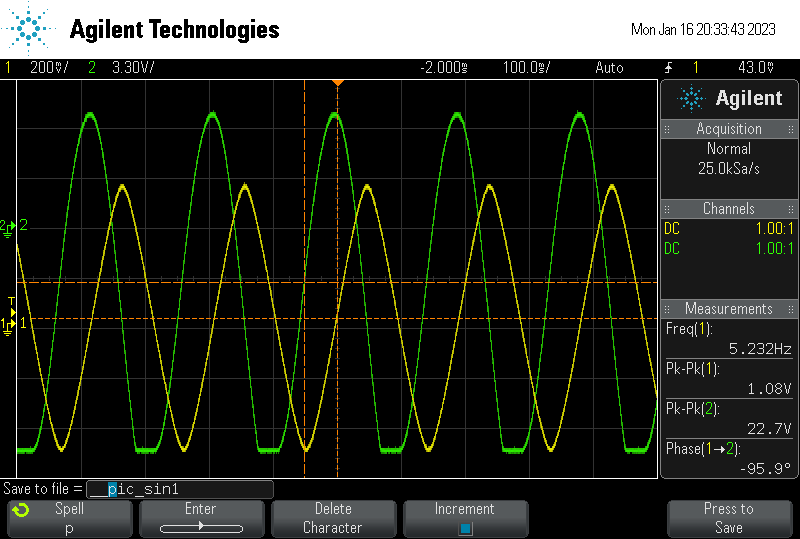
\includegraphics[width=0.5\textwidth]{python/data/__pic_sin1.png}
  \caption{Die Ausgabe des Ausgangssignals für den Integrator inklusive des Sinus-Eingangssignals. }
\label{fig:int_sin}
\end{figure}


\begin{figure}[H]
  \centering
  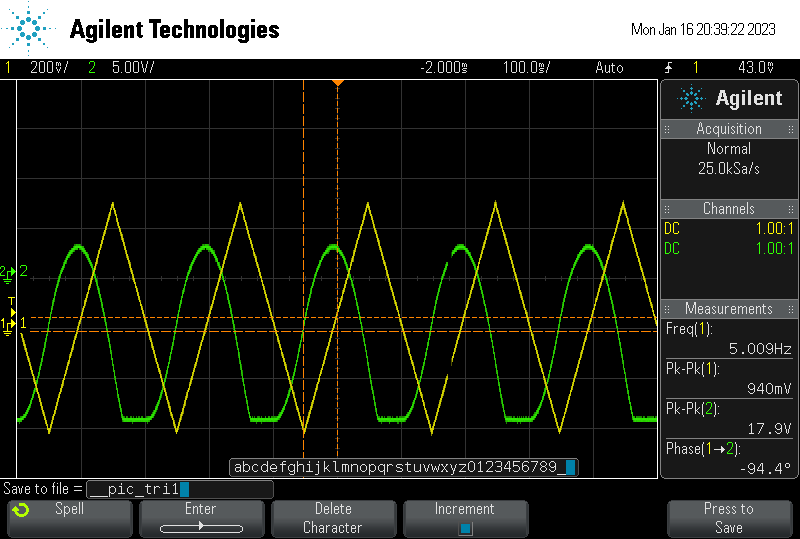
\includegraphics[width=0.5\textwidth]{python/data/__pic_tri1.png}
  \caption{Die Ausgabe des Ausgangssignals für den Integrator inklusive des Dreieck-Eingangssignals. }
\label{fig:int_dre}
\end{figure}


\begin{figure}[H]
  \centering
  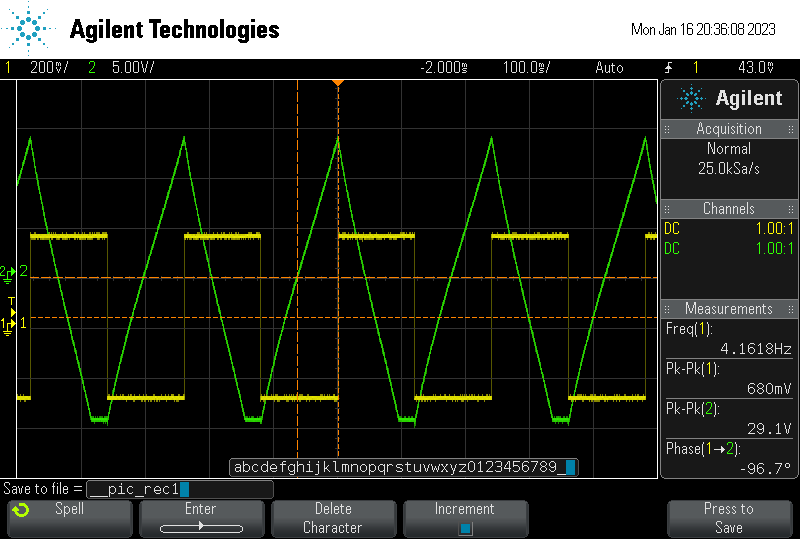
\includegraphics[width=0.5\textwidth]{python/data/__pic_rec1.png}
  \caption{Die Ausgabe des Ausgangssignals für den Integrator inklusive des Rechteck-Eingangssignals. }
\label{fig:int_recht}
\end{figure}


\subsection{Invertierter Differenzierer}

\noindent
Für den Differenzierer mit $R_1 = \SI{100}{\kilo\ohm}$ und dem Kondensator $C = \SI{22}{\nano\farad}$ ist das Vorgehen analog.
Zuerst wird ein Fit auf die, aus den in der Tabelle \ref{tab:diff} zu findenden Messwerte, errechneten Verstärkungsfaktoren bestimmt. 
Anschließend wird über Vergleich mit Gleichung \ref{eqn:dif_RC} $RC$ bestimmt.
Die Parameter der Ausgleichsrechnung wurden zu
\begin{align*}
  m&=\SI{0.95(2)}{}\\
  n&= \SI{-6.02(14)}{}\\
  RC_\t{Diff} &= \SI{2.4(3)}{\milli\second}\; .
\end{align*}
errechnet. Für den theoretischen Wert gilt
\begin{equation*}
  RC_\t{Theo,Diff} = \SI{2.2}{\milli\second}\;. 
\end{equation*}
Der Theoriewert ist inklusive der Ausgleichsgerade und der Messwerte in Abbildung \ref{fig:diff1} zu finden.

\begin{figure}[H]
  \centering
  \includegraphics[width=0.6\textwidth]{build/plots/differenzierer.pdf}
  \caption{Die Messwerte des Verstärkungsfaktors des invertierten Differenzierers gegen die Kreisfrequenz aufgetragen.
  Des Weiteren ist noch eine Theoriekurve und der Fit eingezeichnet.}
\label{fig:diff1}
\end{figure}

\noindent
In den Abbildungen \ref{fig:diff_sin}, \ref{fig:diff_dre} und \ref{fig:diff_recht} sind die wieder die Ausgaben des Oszilloskops 
für eine Sinus-, Dreieck- und Rechteck-Eingangsspannung dargestellt. Dabei sollen die Eingangsspannungen diesmal differenziert werden.
Die Sinusspannung wird also zu einer Kosinusspannung differenziert. Für die Dreiecksspannung wird eine Rechteckspannung erwartet, und für die Rechteckspannung Delta-Peaks.
Allerdings ergibt sich für die Rechteckspannung an den Kanten zwar ein Peak, dieser nimmt danach aber stark oszillierend ungefähr linear ab.
Für die Dreiecksspannung ergibt sich an den Kuspen eine starke Anregung, deren Amplitude stark oszillierend ungefähr exponentiell fällt.


\begin{figure}[H]
  \centering
  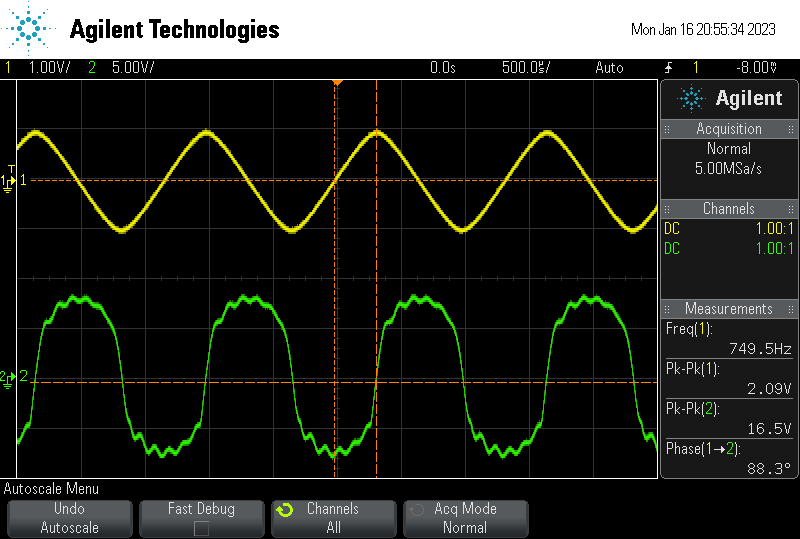
\includegraphics[width=0.5\textwidth]{python/data/__pic_sin2.png}
  \caption{Die Ausgabe des Ausgangssignals für den Differenzierer inklusive des Sinus-Eingangssignals. }
\label{fig:diff_sin}
\end{figure}


\begin{figure}[H]
  \centering
  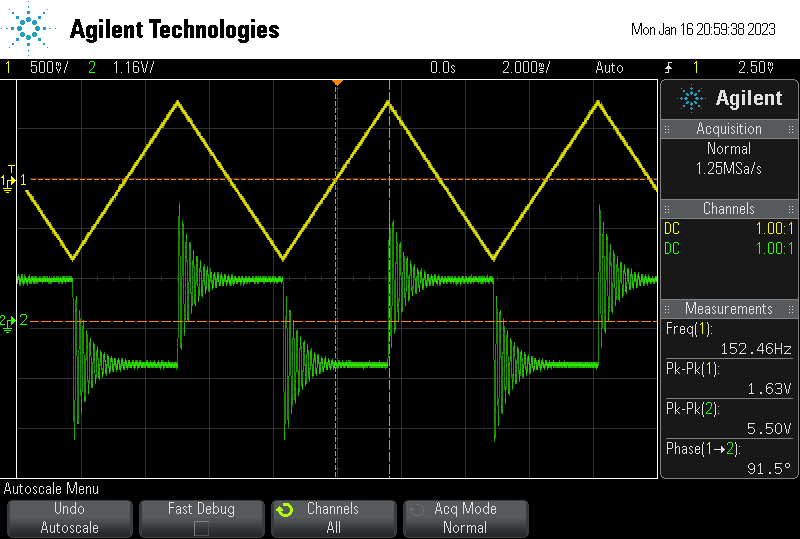
\includegraphics[width=0.5\textwidth]{python/data/__pic_tri2.png}
  \caption{Die Ausgabe des Ausgangssignals für den Differenzierer inklusive des Dreieck-Eingangssignals. }
\label{fig:diff_dre}
\end{figure}


\begin{figure}[H]
  \centering
  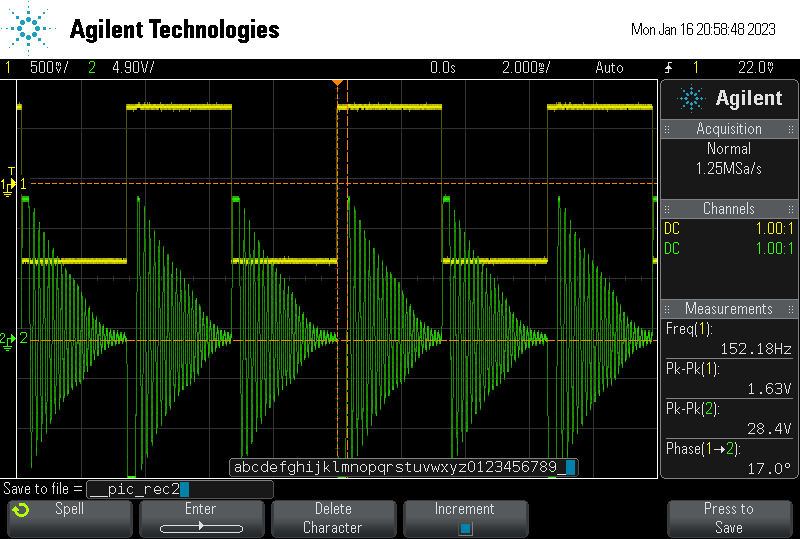
\includegraphics[width=0.5\textwidth]{python/data/__pic_rec2.png}
  \caption{Die Ausgabe des Ausgangssignals für den Differenzierer inklusive des Rechteck-Eingangssignals. }
\label{fig:diff_recht}
\end{figure}


\subsection{Nichtinvertierter Schmitt-Trigger}


\noindent
Für den Schmitt-Trigger werden für ein angelegtes Dreieckssignal die Kippspannungen der Ausgangsspannung abgelesen. 
Die abgelesen Werte sind in Tabelle \ref{tab:schmitt} zu finden, das Messsignal in Abbildung \ref{fig:schmitt}. 
Außerdem wurden die Widerstände $R_1 = \SI{10}{\kilo\ohm}$ und $R_2 = \SI{100}{\kilo\ohm}$ verwendet.
Da die Betriebsspannung $U_\t{b} = \SI{14}{\volt}$, die am Schmitt-Trigger anliegt, symmetrisch ist, berechnet sich die theoretische
Kippspannung $U_\t{Kipp,Theo}$ zu
\begin{equation*}
  U_\t{Kipp,Theo} = \frac{R_1}{R_2} U_\text{b} = \pm \SI{1.4}{\volt}\; .
\end{equation*}

\begin{table}[H]
  \centering
  \small
  \caption{Messdaten zur Bestimmung der Kippspannung des Schmitt-Triggers.}
  \label{tab:schmitt}
  \begin{tabular}{S [table-format=3.3] S [table-format=1.4]}
     \toprule
     {$t \mathbin{\scalebox{1.5} / } \si{\milli\second}$} & $U_\t{Kipp} \mathbin{\scalebox{1.5} / } \si{\volt}$\\
     \midrule
     $\SI{369e-3}{}$ &  1.8625 \\
     1.71  & -1.6625 \\
    -1.04  & -1.675  \\
    -2.35  &  1.8625 \\
    \bottomrule
  \end{tabular}
  \end{table} 

  \noindent
  Über das Mitteln der in der Tabelle aufgeführten positiven und negativen Kippspannungen ergibt sich
  \begin{align*}
    U_\t{Kipp,+} &= \SI{1.8625}{\volt}\\
    U_\t{Kipp,-} &= \SI{-1.669(6)}{\volt}\;.
  \end{align*}


\begin{figure}[H]
  \centering
  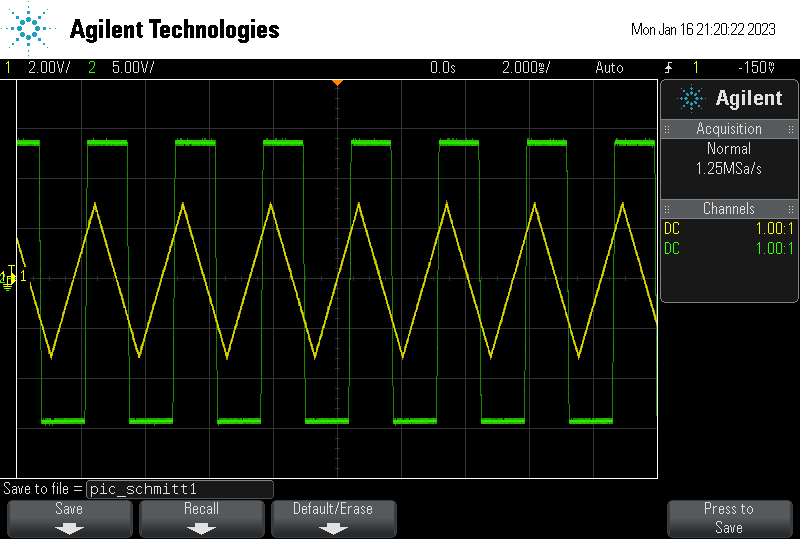
\includegraphics[width=0.5\textwidth]{python/data/pic_schmitt1.png}
  \caption{Die Ausgabe der Dreieckseingansspannung und der Rechteckausgangsspannung die zur Bestimmung der Kippspannung des Schmitt-Triggers verwendet wird. }
\label{fig:schmitt}
\end{figure}


\subsection{Signalgenerator}

\noindent
Zuletzt wird hinter dem Schmitt-Trigger noch ein Integrator aufgebaut, um ein Signal zu erzeugen.
Dafür werden die Bauteile $R_1 = \SI{10}{\kilo\ohm}$, $R_2 = \SI{100}{\kilo\ohm}$, $R_3 = \SI{1}{\kilo\ohm}$, $C = \SI{1}{\micro\farad}$ verwendet.
Darüber lassen sich die theoretische maximale Amplitude $U_\t{max,Theo}$ und die theoretische Frequenz $f_\t{Theo}$ des Dreieckssignals bestimmen.
Diese ergiben sich zu
\begin{align*}
  U_\t{max,Theo} &= U_\t{b} \frac{R_1}{R_2} &= \SI{1.375}{\volt} \\
  f_\t{Theo} &= \frac{R_2}{4 R_1 R_3 C}     &= \SI{2.5}{\kilo\hertz}  \; .
\end{align*}
Dabei wurde $U_\t{a} = \SI{13.75}{\volt}$ als halbe \enquote{Peak-to-Peak}-Amplitude des Rechtecksignals aus Abbildung \ref{fig:sig} abgelesen.
Für die mit dem Oszilloskop bestimmten Werte gilt 
\begin{align*}
  U_\t{max,mess}  &= \SI{2.65}{\volt}\\
  f_\t{mess}  &= \SI{1.64}{\kilo\hertz} \; .
\end{align*} 

\begin{figure}[H]
  \centering
  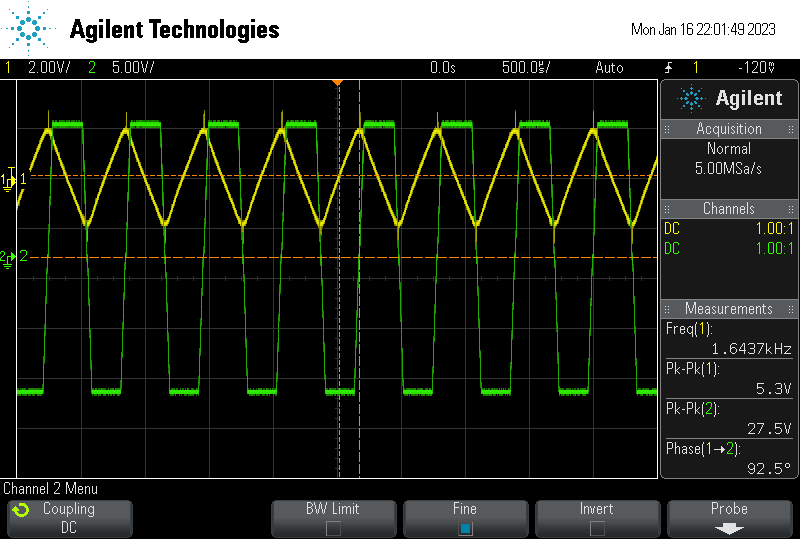
\includegraphics[width=0.5\textwidth]{python/data/pic_signal1.png}
  \caption{Die Ausgabe des Signalgenerators, wobei die Rechteckspannung hinter dem Schmitt-Trigger und die Dreiecksspannung am Ende des Generators abgegriffen wurden. }
\label{fig:sig}
\end{figure}

